\documentclass{standalone}
\usepackage{graphicx}	
\usepackage{amssymb, amsmath}
\usepackage{color}

\usepackage{tikz}
\usetikzlibrary{intersections, backgrounds, math}
\usepackage{pgfmath}

\definecolor{light}{RGB}{254, 245, 144}
\definecolor{dark}{RGB}{238, 202, 2}
\definecolor{gray70}{gray}{0.7}

\begin{document}

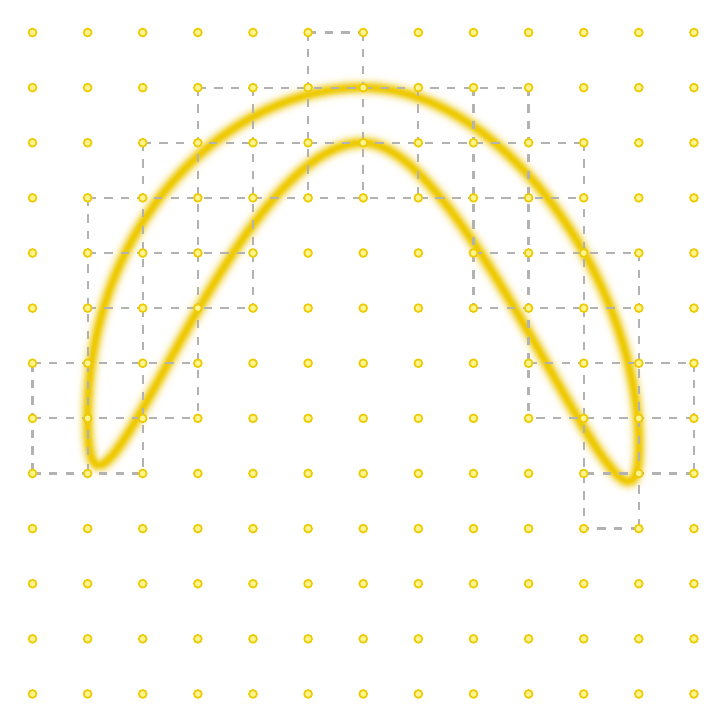
\begin{tikzpicture}[scale=0.35, thick]

    \foreach \i in {1, 0.99, ..., 0} {
            \pgfmathsetmacro{\prop}{100 * exp(-20.0 * \i * \i)};
            \colorlet{custom}{dark!\prop!white};
            \draw[line width={20
                        * \i}, color=custom]
            (0, 10) .. controls (5, 10) and (10, 3) .. (10, -3)
            .. controls (10, -9) and (4, 8) .. (0, 8)
            .. controls (-5, 8) and (-10, -9) .. (-10, -2)
            .. controls (-10, 5) and (-5, 10) .. (0, 10);
        }


    \draw[dashed, color=gray70] (-12, 0) -- (-12, -4);
    \draw[dashed, color=gray70] (-10, 6) -- (-10, -4);
    \draw[dashed, color=gray70] (-8, 8) -- (-8, -4);
    \draw[dashed, color=gray70] (-10, 4) -- (-4, 4);
    \draw[dashed, color=gray70] (-10, 2) -- (-4, 2);
    \draw[dashed, color=gray70] (-12, 0) -- (-6, 0);
    \draw[dashed, color=gray70] (-12, -2) -- (-6, -2);
    \draw[dashed, color=gray70] (-12, -4) -- (-8, -4);

    \draw[dashed, color=gray70] (8, 8) -- (8, -6);
    \draw[dashed, color=gray70] (10, 4) -- (10, -6);
    \draw[dashed, color=gray70] (10, -6) -- (8, -6);
    \draw[dashed, color=gray70] (12, 0) -- (12, -4);
    \draw[dashed, color=gray70] (12, -2) -- (6, -2);
    \draw[dashed, color=gray70] (6, 0) -- (12, 0);
    \draw[dashed, color=gray70] (4, 2) -- (10, 2);
    \draw[dashed, color=gray70] (4, 4) -- (10, 4);
    \draw[dashed, color=gray70] (2, 6) -- (8, 6);
    \draw[dashed, color=gray70] (-8, 8) -- (8, 8);
    \draw[dashed, color=gray70] (-6, 10) -- (6, 10);
    \draw[dashed, color=gray70] (-2, 12) -- (0, 12);
    \draw[dashed, color=gray70] (-6, 10) -- (-6, -2);
    \draw[dashed, color=gray70] (-4, 10) -- (-4, 2);
    \draw[dashed, color=gray70] (-2, 12) -- (-2, 6);
    \draw[dashed, color=gray70] (0, 12) -- (0, 6);
    \draw[dashed, color=gray70] (2, 10) -- (2, 6);
    \draw[dashed, color=gray70] (-10, 6) -- (6, 6);
    \draw[dashed, color=gray70] (4, 10) -- (4, 2);
    \draw[dashed, color=gray70] (6, 10) -- (6, -2);
    \draw[dashed, color=gray70] (-6, 10) -- (-6, 8);
    \draw[dashed, color=gray70] (12, -4) -- (8, -4);










    \foreach \x in {-12, -10, ..., 12} {
            \foreach \y in {-12, -10, ..., 12} {
                    \fill[color=dark] (\x, \y) circle (5pt);
                    \fill[color=light] (\x, \y) circle (3pt);
                }
        }

\end{tikzpicture}

\end{document}